%%%%%%%%%%%%%%%%%%%%%%%%%%%%%%%%%%%%%%%%%
% Design based on a template by Roberto and following the format of
% the xmipp tutorials. In turn, they seem to be based on a template
% from http://www.latextemplates.com
%%%%%%%%%%%%%%%%%%%%%%%%%%%%%%%%%%%%%%%%%

%----------------------------------------------------------------------------------------
%	PACKAGES AND OTHER DOCUMENT CONFIGURATIONS
%----------------------------------------------------------------------------------------

\documentclass[12pt]{article} % Default font size is 12pt, it can be changed here
\usepackage[english]{babel}
\usepackage[utf8]{inputenc}
\usepackage{listings} % To include source code
\usepackage{caption}
\usepackage{geometry} % Required to change the page size to A4
%\geometry{a4paper} % Set the page size to be A4 as opposed to the default US Letter
\usepackage{framed}
\usepackage{url}
\usepackage{graphicx} % Required for including pictures
\usepackage{natbib}
\usepackage{float} % Allows putting an [H] in \begin{figure} to specify the exact location of the figure
\usepackage{hyperref}
\usepackage{menukeys}
\usepackage{array}
\usepackage{fancyhdr}
\usepackage{marvosym}%smileys\Smiley{} \Frowny{}
\usepackage{etoolbox}
\usepackage{listings}
\usepackage{makecell}
\usepackage{marginnote}
\usepackage{soul}
\usepackage[toc,page]{appendix}
\usepackage{caption}
\sethlcolor{yellow}

%\renewcommand{\hl}[1]{#1}
%pdflatex -jobname=students '\def\student{}\input{main}'
%pdflatex -jobname=teachers '\def\teachers{}\input{main}'
%  \ifdef{\teachers}
%  {Content for teachers}
%  {Content for students}
\newcommand{\ttt}[1]{\texttt{#1}}
\newcommand{\iii}[1]{\textit{#1}}
\newcommand{\ra}{$\rightarrow$}
\pagestyle{fancy}
\fancyhf{}
\fancyhead[RO]{{Model Building}}
\fancyhead[LO]{Scipion}
%\fancyhead[RO]{{\leftmark}}
\fancyfoot[RO]{\thepage}

\linespread{1.2} % Line spacing

%\setlength\parindent{0pt} % Uncomment to remove all indentation from paragraphs

\newcommand{\scipion}{\textsc{Scipion} }
\newenvironment{command}{\tt\begin{quote}}{\end{quote}}
\newcommand{\comm}[1]{\texttt{#1}}

\newcommand{\imgfig}[3]{\begin{figure}[H]\centering \
\includegraphics[scale=#2]{images/#1} \caption{#3} \end{figure}}

\newcommand{\proto}[1]{\textit{\textbf{#1}}}
\newcommand{\popt}[1]{\textit{#1}}
\newcommand{\pval}[1]{\texttt{#1}}

\newcommand\tstrut{\rule{0pt}{2.4ex}}
\newcommand\bstrut{\rule[-1.0ex]{0pt}{0pt}}

\def \humanAdenoMap {7034}%5172

\begin{document}

%----------------------------------------------------------------------------------------
%	TITLE PAGE
%----------------------------------------------------------------------------------------

\begin{titlepage}

% New command for horizontal lines. Change thickness here.
\newcommand{\HRule}{\rule{\linewidth}{0.5mm}}

\center % Center everything on the page


\includegraphics{images/scipion_logo.png}

{\large Scipion Tutorial Series}\\[1.0cm]

\textsc{\LARGE National Center for Biotechnology}\\[0.5cm]
\textsc{\Large Biocomputing Unit}\\[0.15cm]

\HRule\\[0.4cm]
{ \huge \bfseries Model Building Basic}\\ % Title of your document
\HRule \\[0.5cm]
%{\large \today}\\[3cm] % Date, change the \today to a set date if you want to be precise
\begin{center}
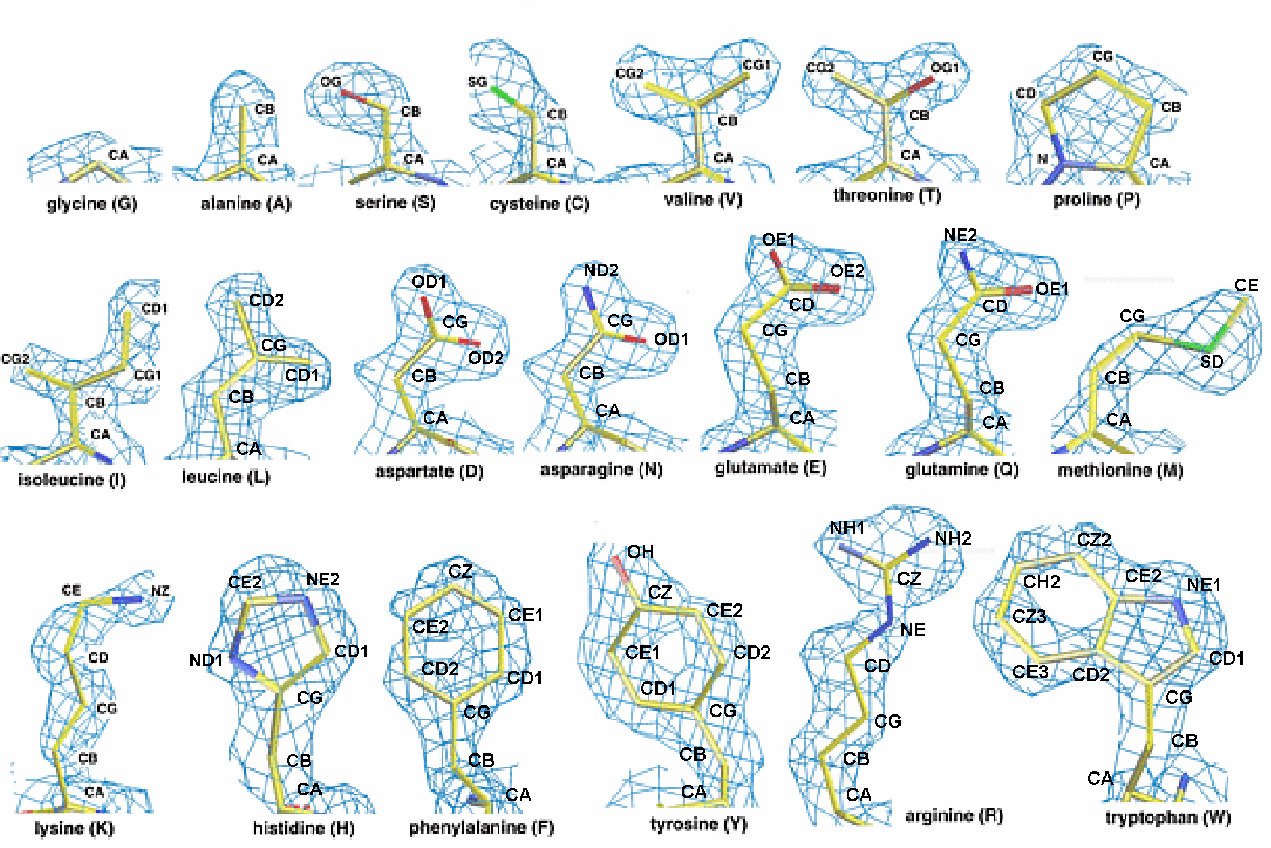
\includegraphics[width=0.70\textwidth]{{images/aadensity}.png}\\
Density for amino acid side chains from an experimental electron density map at 1.5 \AA~resolution (http://people.mbi.ucla.edu/sawaya/m230d/Modelbuilding/modelbuilding.html)\end{center}

%\vfill % Fill the rest of the page with whitespace
%\begin{minipage}{0.4\textwidth}
\begin{flushright}
 \large
%\emph{Author:}\\
  \textsc{Roberto Marabini AND Marta Martínez} % Your name
\end{flushright}
%\end{minipage}

\end{titlepage}


%----------------------------------------------------------------------------------------
%	OBJETIVOS
%----------------------------------------------------------------------------------------


\subsection*{Intended audience}
The recent rapid development of single-particle electron cryo-microscopy (cryo-EM) allows structures to be solved by this method at resolutions close to 3\AA.  Providing a basic introduction to model building, this tutorial shows the initial workflow aimed at obtaining high-quality atomic models from cryo-EM data by using Scipion software framework. %tomography in  electron microscopy with special emphasis in basic image processing. The tutorial requires matlab but does not assume any programing skills. 


\subsection*{We'd like to hear from you}

We have tested and verified the different steps described in this demo
to the best of our knowledge, but since our programs are in continuous
development you may find inaccuracies and errors in this text. Please
let us know about any errors, as well as your suggestions for
future editions, by writing to
\href{mailto:scipion@cnb.csic.es}{scipion@cnb.csic.es}.


\subsection*{Requirements}

This tutorial requires, in addition to $Scipion$,  the \textit{CCP4 suite} including $refmac$ and $coot$, the \textit{PHENIX suite} and $USCF Chimera$. Basic knowledge of $USCF Chimera$ and $Scipion$ is assumed. Warning: all versions of $refmac$ are not suitable for EM data.

\newpage


%----------------------------------------------------------------------------------------
%	TABLE OF CONTENTS
%----------------------------------------------------------------------------------------

\tableofcontents % Include a table of contents

\newpage % Begins on a new page instead of on the same page as the table of contents


\section{Introduction to Model building}

\begin{itemize}
 \item Definition:\\Model building is the process that allows getting the atomic interpretation of a electron density map. Although a electron density volume can be obtained from different methodologies, in this $Scipion$ tutorial we focus in maps obtained by cryo-EM. As an example of these maps, Fig. 1 details the input electron density volume (a), as well as the output hemoglobin tetramer atomic model (b) obtained by the model building process. Since high quality atomic structures are essential to accomplish detailed mechanistic studies and to seek inhibitor drugs of macromolecules, the main aim of model building is obtaining reliable structures of these macromolecules. 
 

\begin{figure}[H]
 \centering
 \captionsetup{width=.8\linewidth}  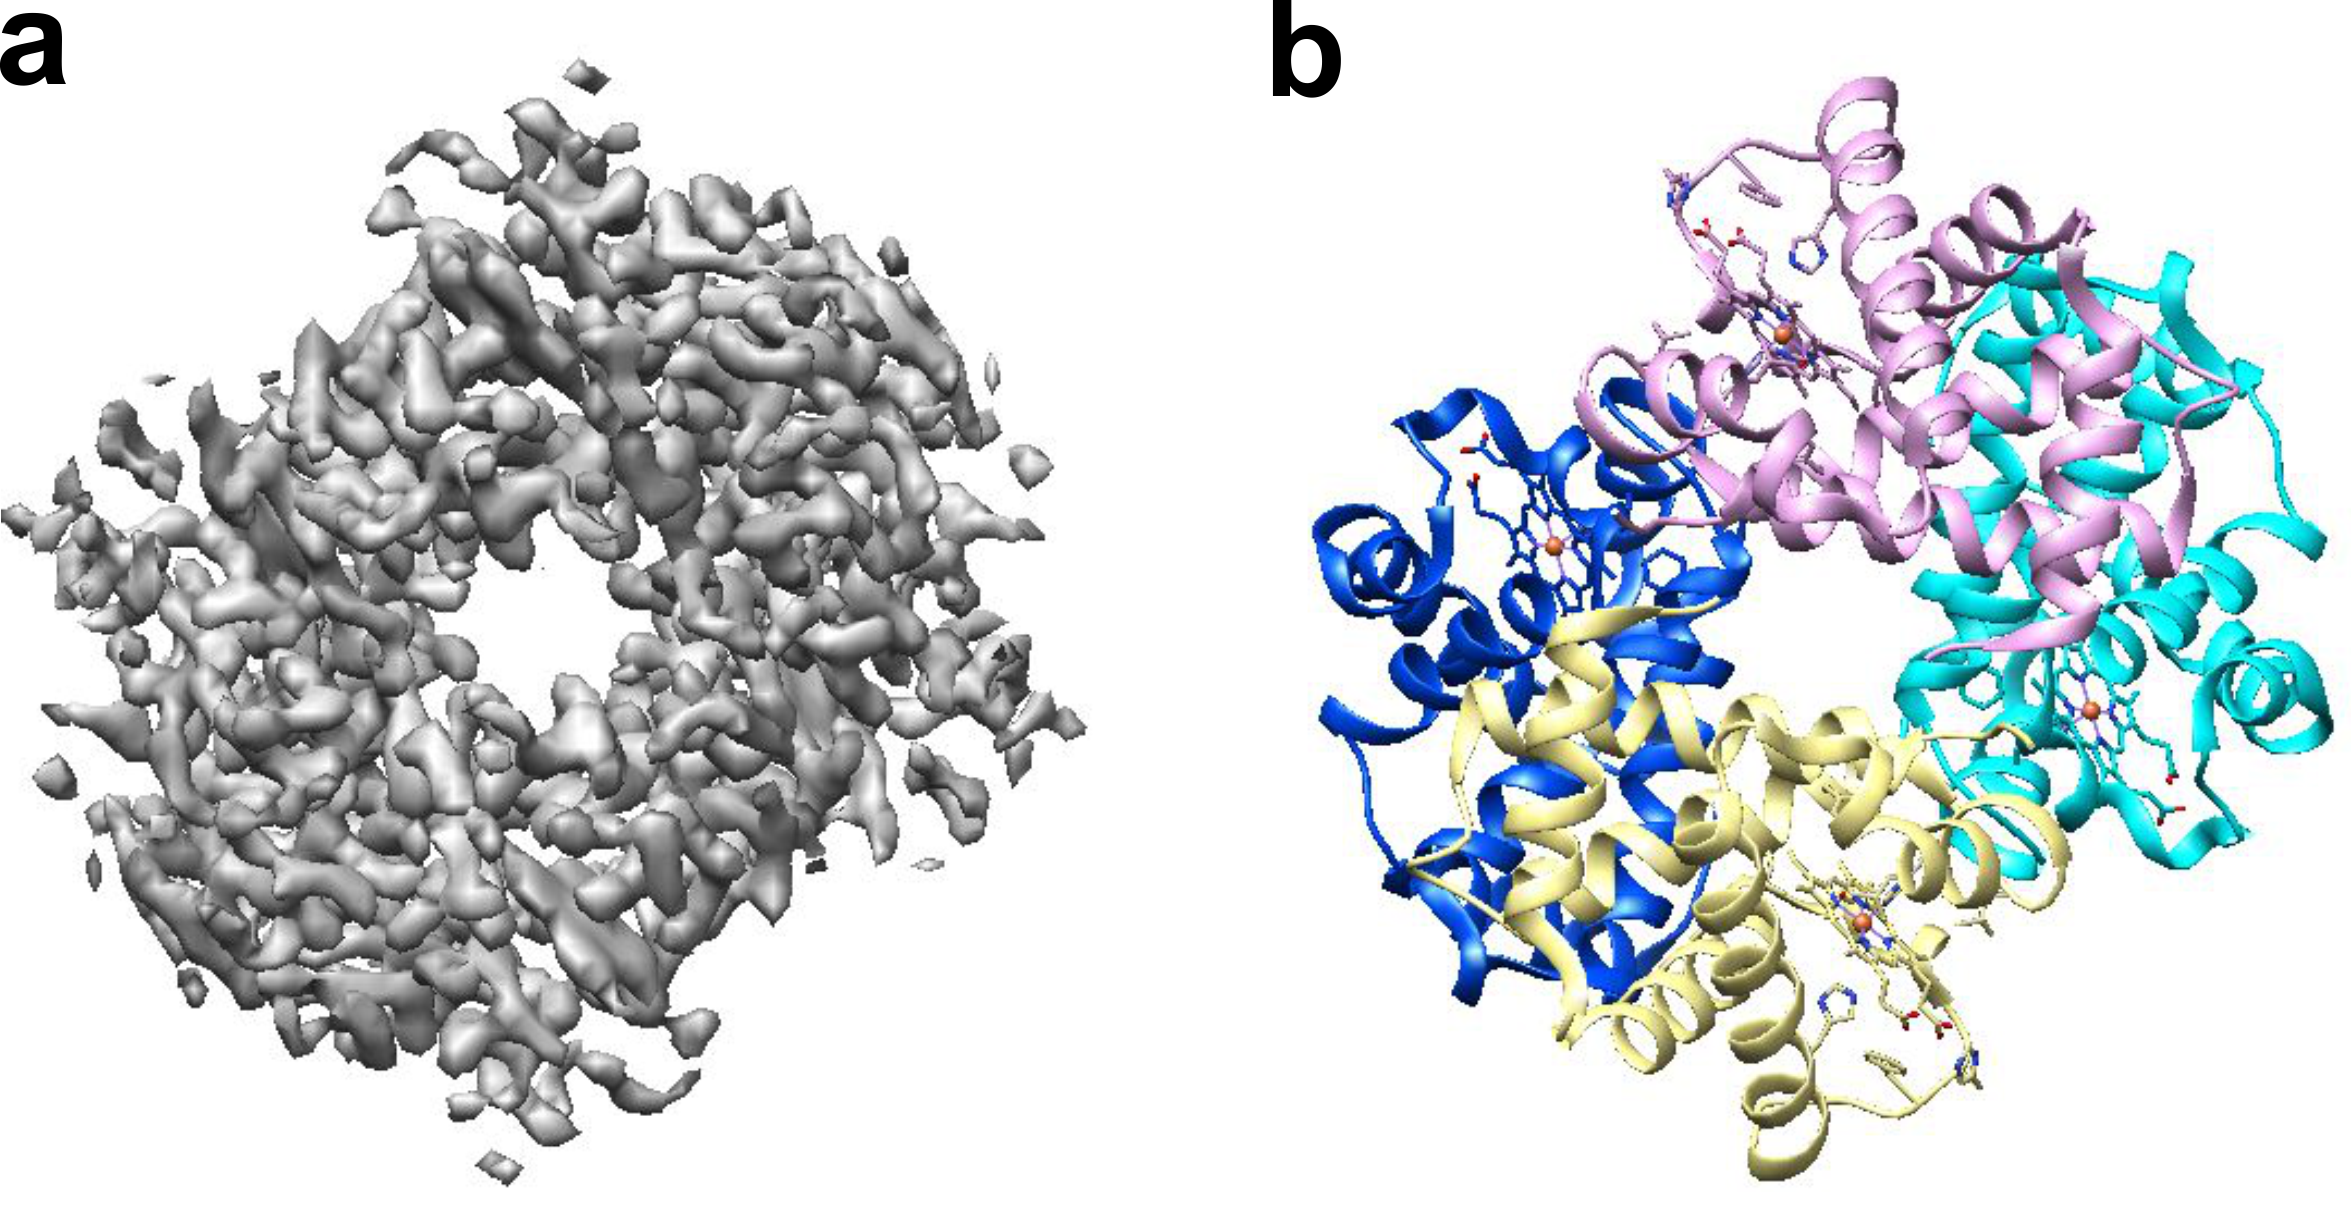
\includegraphics[width=0.6\textwidth]
  {{Images/Fig1}.png}
  \caption{Hemoglobin tetramer (Danev and Baumeister, 2016). a) Electron density map at 3.2\AA\ resolution obtained by Cryo-EM single particle analysis with Volta phase plate. b) Atomic structure model inferred from the electron density volume.}
  \label{fig:model_building_example}
  \end{figure} 
 

\item Relevance of cryo-EM map resolution:\\Model building process is extraordinarily limited by the resolution of the starting cryo-EM density map. The lower the resolution, the more detailed and reliable atomic structure will be obtained. Fortunately, single-particle cryo-EM is undergoing in this decade a resolution revolution that has allowed the structures of macromolecules to be solved at near-atomic resolution. The density map is thus sufficiently resolved to build the atomic model. As a general rule, at resolutions of 4.5\AA\ the molecule backbone can be inferred based on the map alone, and resolutions lower than 4\AA\ allow to trace some residue side chains. 
 \item Model building workflow:\\The set of succesive tasks aimed to get the atomic interpretation of electron density maps are kown as model building workflow. Main steps names of this general workflow are detailed top-to-bottom in Fig. 2. Taks' names and tools required are highlighted in green in the left side of the Fig. In short, this workflow considers as input the lower asymmetrical element (unit cell) of the starting volume and the sequence of each individual structural element (from 1 to n). These sequences are used to get the initial models, $de novo$ or by prediction based in homologous structures. Initial model of each individual structural element has to be fitted to the unit cell volume, and then refined accordig to the its fitted volume. Since the double refinement in real and reciprocal spaces seems to improve protein models (Brown $et al.$, 2015; Tools for macromolecular model building and refinement into electron cryo-microscopy reconstructions), these two steps of refinement are included in the workflow. Once refined, the geometry of each individual structure has to be validated regarding the starting volume. The last two steps of refinement and validation will be applied globally to the whole set of structures contained in that volume to avoid forbidden steric overlaps among them. In the reconstruction of the whole volume, borders between adjacent unit cells will be checked in this same way. 
 
 In this basic tutorial of model building we are considering every step of the general workflow, except the $de novo$ modeling step because the appropriate tools to accomplish this type of modeling are not still implemented in $Scipion$. 
 
\begin{figure}[H]
 \centering
 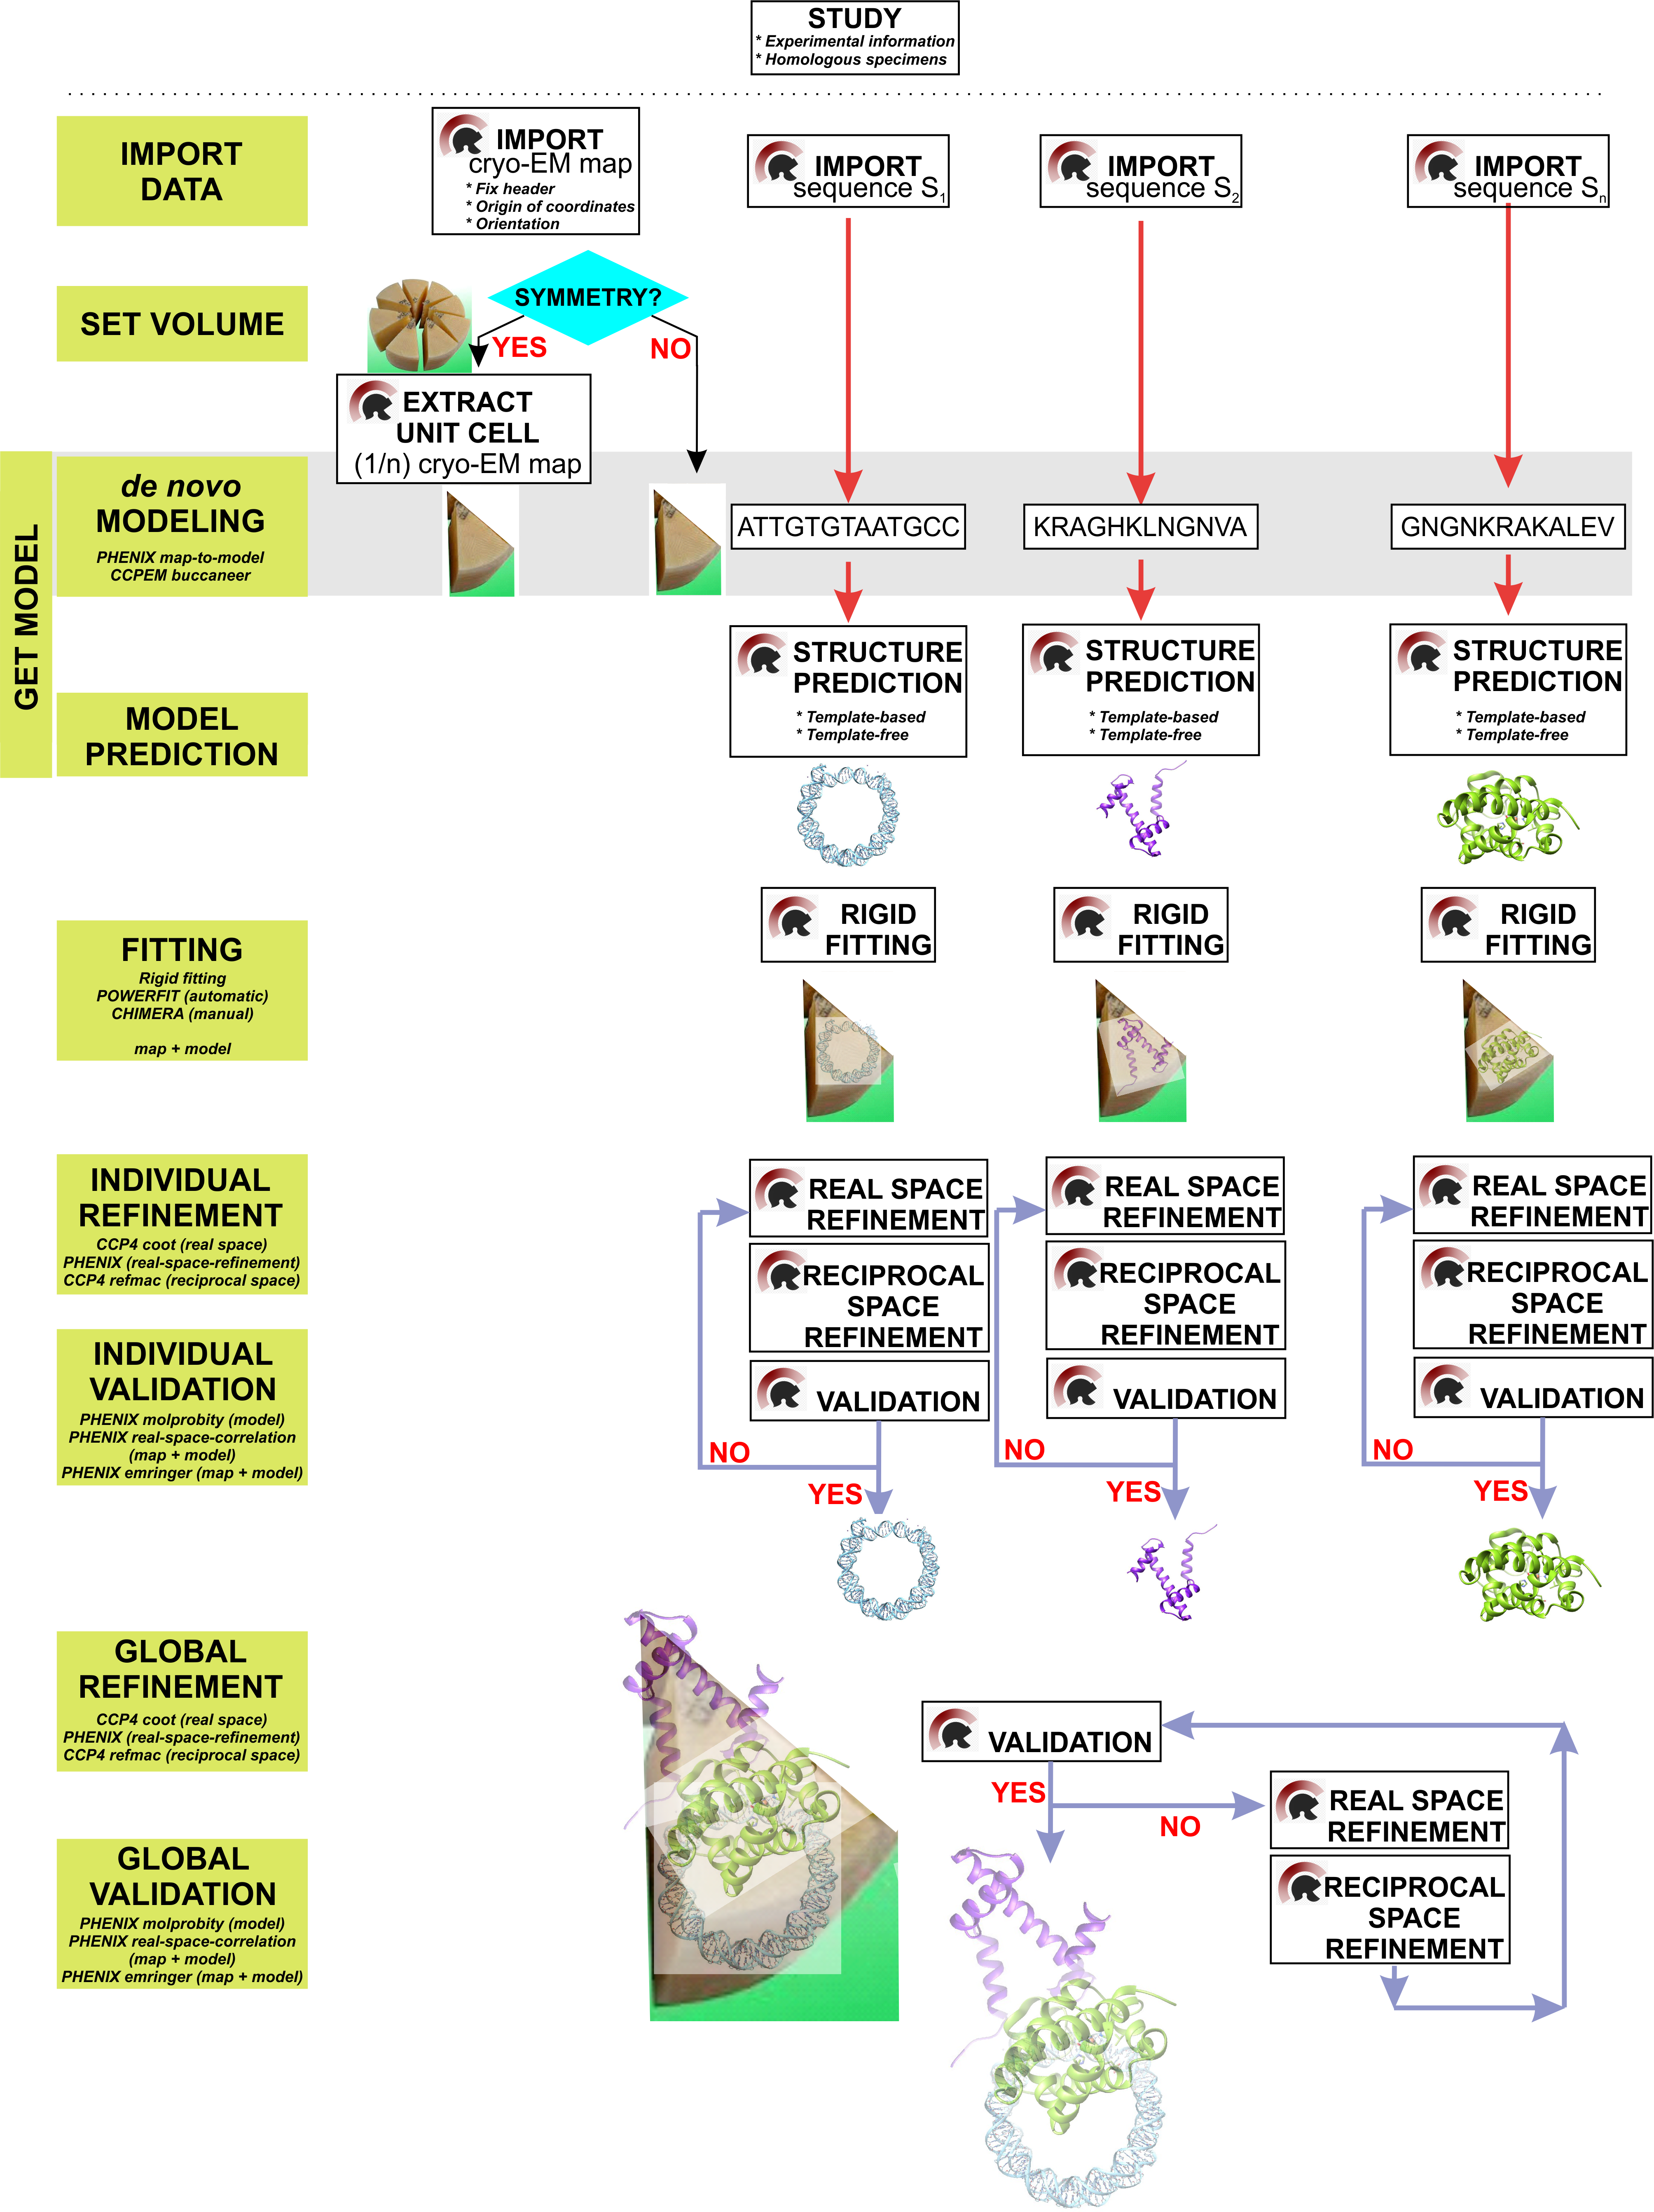
\includegraphics[width=0.95\textwidth]
  {{Images/Fig2}.png}
  \caption{General Model Building Workflow.}
  \label{fig:model_building_workflow}
  \end{figure} 
  
\end{itemize}  

\section{Particular problem to be solved: Hemoglobin}
Due to the basic nature of this tutorial, the small Hemoglobin macromolecule (~64 KDa) has been selected to model its atomic structure. 

The metalloprotein Hemoglobin is the iron-containing protein able to transport oxygen, essential to get energy from aerobic metabolic reactions, through the red blood cells of almost every vertebrate. The first atomic structure of hemoglobin was determined in 1959 by X-ray crystallography (Perutz $et al.$, 1960; Structure of haemoglobin: a three-dimensional Fourier synthesis at 5.5-\AA\ resolution, obtained by X-ray analysis).

\begin{appendices}
\section{Input volume protocol}

\section{Input pdb protocol}


\marginnote{swissmodel}[1cm]
When predicting by homology a structure is constructed by aligning a target protein sequence with known template structures. The protein sequence can be obtained from many sources, for example NCBI or UniProt. The quality of a structure depends upon the similarity between the target sequence and the database sharing highest similarity is aligned. 

Esto es otro parrafo


\end{appendices}

\end{document}
